% !TEX TS-program = pdflatex
% !TEX encoding = UTF-8 Unicode

% This is a simple template for a LaTeX document using the "article" class.
% See "book", "report", "letter" for other types of document.

\documentclass[12pt]{article} % use larger type; default would be 10pt






%%% PAGE DIMENSIONS
\usepackage{makeidx}
\usepackage{hyperref}
\usepackage{listings}
\usepackage{color}
\usepackage[margin=0.75in]{geometry} % to change the page dimensions
\geometry{a4paper} % or letterpaper (US) or a5paper or....
\lstset{
language=Java,
basicstyle=\small\sffamily,
numbers=left,
numberstyle=\tiny,
frame=tb,
columns=fullflexible,
showstringspaces=false
}
\usepackage[pdftex]{graphicx} % support the \includegraphics command and options

\usepackage{array} % for better arrays (eg matrices) in maths
\usepackage{verbatim} % adds environment for commenting out blocks of text & for better verbatim
%\usepackage{subfig} % make it possible to include more than one captioned figure/table in a single float
% These packages are all incorporated in the memoir class to one degree or another...

%%% HEADERS & FOOTERS
\usepackage{fancyhdr} % This should be set AFTER setting up the page geometry


\newcommand{\HRule}{\rule{\linewidth}{0.5mm}}

\title{}
\begin{document}
\maketitle
\begin{titlepage}

\begin{center}


% Upper part of the page

\includegraphics[scale=0.75]{RVCE.png}\\[1cm]    

\textsc{\LARGE  RV College of Engineering}\\[0.5cm]
\large{Department of Computer Science}\\[1cm]
\textsc{\Large }\\[0.5cm]

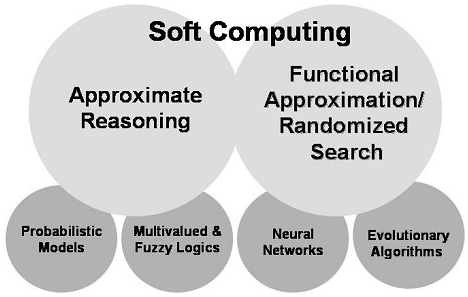
\includegraphics[scale=1]{softee.png}\\[1cm]    

% Title
\HRule \\[0.4cm]
{  \huge\bfseries Soft Set Theory for Soft Computing }\\[0.4cm]

\HRule \\[1cm]

% Author and supervisor
\begin{minipage}{0.8\textwidth}
\begin{flushleft} \large
\emph{By:}\\
Samir \textsc{Sheriff} [1RV09CS093]\\
Satvik \textsc{N} [1RV09CS095]\\


\end{flushleft}
\end{minipage}
\vfill

% Bottom of the page
{\large}

\end{center}

\end{titlepage}



\maketitle
\setcounter{secnumdepth}{1}

\section{Introduction}
Molodtsov initiated the concept of soft set as a new mathematical tool for dealing with uncertainties. Most of our traditional tools for formal modeling, reasoning and computing are crisp, deterministic and precise in character. However, there are many complicated problems in economics,
engineering, environment, social science, medical science etc.
that involve uncertainties. The Theory of Probability, Theory of
Fuzzy Sets,Theory of Intuitionistic Fuzzy Sets,Theory of Vague
Sets, Theory of Interval Mathematics and Theory of Rough Sets
are considered as mathematical tools for dealing with
uncertainties.

In 1999, Molodstov pointed out that these
theories which are considered as mathematical tools for dealing
with uncertainties, have certain limitations. He further pointed
out that the reason for these limitations is, possibly, the
inadequacy of the parameterization tool of the theory. The Soft
Set Theory introduced by Molodstov is quite different from
these theories in this context. The absence of any restrictions on
the approximate description in Soft Set Theory makes this
theory very convenient and easily applicable. Fuzzy set theory
proposed by Professor L. A. Zadeh in 1965 is considered as a
special case of the soft sets.

Current and soft mathematics can
co-exist and can be used consistently to solve real
world problems.


\section{Soft Computing}
\subsection{Definition}
Soft computing differs from conventional (hard) computing in that, unlike hard computing, it is tolerant of imprecision, uncertainty, partial truth, and approximation. In effect, the role model for soft computing is the human mind. The guiding principle of soft computing is: Exploit the tolerance for imprecision, uncertainty, partial truth, and approximation to achieve tractability, robustness and low solution cost. The basic ideas underlying soft computing in its current incarnation have links to many earlier influences, among them Zadeh's 1965 paper on fuzzy sets; the 1973 paper on the analysis of complex systems and decision processes; and the 1979 report (1981 paper) on possibility theory and soft data analysis. The inclusion of neural computing and genetic computing in soft computing came at a later point.

\subsection{Words of Wisdom}
\textit{"Basically, soft computing is not a homogeneous body of concepts and techniques. Rather, it is a partnership of distinct methods that in one way or another conform to its guiding principle. At this juncture, the dominant aim of soft computing is to exploit the tolerance for imprecision and uncertainty to achieve tractability, robustness and low solutions cost. The principal constituents of soft computing are fuzzy logic, neurocomputing, and probabilistic reasoning, with the latter subsuming genetic algorithms, belief networks, chaotic systems, and parts of learning theory. In the partnership of fuzzy logic, neurocomputing, and probabilistic reasoning, fuzzy logic is mainly concerned with imprecision and approximate reasoning; neurocomputing with learning and curve-fitting; and probabilistic reasoning with uncertainty and belief propagation".}

\subsection{Components of Soft Computing}
At this juncture, the principal constituents of Soft Computing (SC) are Fuzzy Logic (FL), Neural Computing (NC), Evolutionary Computation (EC) Machine Learning (ML) and Probabilistic Reasoning (PR), with the latter subsuming belief networks, chaos theory and parts of learning theory. What is important to note is that soft computing is not a melange. Rather, it is a partnership in which each of the partners contributes a distinct methodology for addressing problems in its domain. In this perspective, the principal constituent methodologies in SC are complementary rather than competitive. Furthermore, soft computing may be viewed as a foundation component for the emerging field of conceptual intelligence.

Components of soft computing include:
\begin{itemize}

\item{Neural networks (NN)}
\item{Fuzzy logics (FL)}
\item{Evolutionary computation (EC), including:}
\begin{itemize}
\item{Evolutionary algorithms}
\begin{itemize}
\item{Genetic algorithms}
\item{Differential evolution}
\end{itemize}
\item{Metaheuristic and Swarm Intelligence}
\begin{itemize}
\item{Ant colony optimization}
\item{Bees algorithms}
\item{Bat algorithm}
\item{Cuckoo search}
\item{Harmony search}
\item{Firefly algorithm}
\item{Artificial immune systems}
\item{Particle swarm optimization}
\end{itemize}
\end{itemize}
\item{Ideas about probability including Bayesian networks}
\item{Chaos theory}
\item{Perceptron}

\end{itemize}
Generally speaking, soft computing techniques resemble biological processes more closely than traditional techniques, which are largely based on formal logical systems, such as sentential logic and predicate logic, or rely heavily on computer-aided numerical analysis (as in finite element analysis). Soft computing techniques are intended to complement each other.
Unlike hard computing schemes, which strive for exactness and full truth, soft computing techniques exploit the given tolerance of imprecision, partial truth, and uncertainty for a particular problem. Another common contrast comes from the observation that inductive reasoning plays a larger role in soft computing than in hard computing.



\section{Soft Set Theory}

\subsection{Structured Subsets}
According to the authors of this oh so marvelous paper, ideal membership functions for real world fuzzy sets are made from elastic material, because fuzzy sets should be able to tolerate certain
amount of perturbation or stretching. Mathematically, each perturbation is a new function, that consists of a set of functions,
each of which can be continuously stretched into
another function. Such a set of functions is a highly
structured subset of membership function space. 

\subsection{Soft Sets}
A fuzzy set, which is also called, in different parts of the world, a soft set, is an \textit{“abstract structured set”} of
membership function space. Such a structured subset
may be an equivalence class, a neighborhood, or
fuzzified structures in the membership function space. Soft sets are intended to capture and to defuse the conflicts among existing fuzzy theories. So a fuzzy set could be defined by 
\begin{enumerate}
\item{A collection of membership functions}
\item{that should be able to transform among themselves}
\end{enumerate}


\subsection{Neighbourhood Systems}
It is an abstraction of “near” or “negligible distances” in
geometry. A neighborhood system is an association that
assigns each datum a list of data that may or may not
contain the datum. It is natural and implementable, and used for  approximate retrieval in databases and approximate reasoning in knowledge bases

The central notion here is neighborhood systems. It
is an abstraction of “near” or “negligible distances” in
geometry. A neighborhood system is an association that
assigns each datum a list of data that may or may not
contain the datum. It is natural and implementable. So current and soft mathematics can
co-exist and can be used consistently to solve real
world problems.

Neighborhood systems express the semantics of
nearby spaces. Let p be an object (or datum) in the universe or
space X. 

\begin{itemize}
\item{A neighborhood, denoted by N(p), or simply N,
of p is a non-empty subset of X, which may or
may not contain the object p.}
\item{Any subset that contains a
neighborhood is a neighborhood.}
\item{A neighborhood
system of object p, denoted by NS(p), is a non-empty
maximal family of neighborhoods of p.}
\item{A neighborhood system of X, denoted by NS(X) is the
collection of NS (p) for all objects p in X.}
\item{If a
neighborhood system NS(X) that satisfies certain
axioms, then X is a topological space. In
general, X is a Frechet (V) space.}
\item{From this view, rough set theory is a special case of the
neighborhood system theory.}
\end{itemize}


\subsection{Soft sets, defined using Neighbourhood Systems}
A real world fuzzy set is defined abstractly by a neighborhood systems of membership function space. Neighborhood systems translate the real world problem into a mathematical problem. So our ultimate goal is to axiomatize fuzzy sets through such neighborhood
systems.


\subsection{Membership Function Space}
Let U be the universe of discourse, and let
FX : U \begin{math} \rightarrow \end{math} M
be a map, where M is, in general, a membership space. 

FX is called a membership function; FX(x) is called the grade or degree of membership of x \begin{math} \in \end{math} U. 

If M is the set of two elements $\{$0, 1$\}$, then FX is the
characteristic function of a classical crispy set. If M is a
unit interval [0, 1], then FX is the membership function of a
classical fuzzy set.

Let F be a collection of fuzzy sets on U. Each fuzzy set is defined by a neighborhood (may be a singleton) in the membership function space; let Col be a neighborhood system. MF(U) is the total union of all membership functions representing F, namely the union of members in Col :
MF(U) = \begin{math} \bigcup \end{math} Col \\
Col is a neighborhood system on MF(U).


\subsection{Types of Soft Sets}
Depending on the nature of Col, we have various types of fuzzy sets (sofsets).
\begin{enumerate}
\item{\textbf{W-Sofset} - Weighted Soft Set (Mathematical Soft
Set or Quantitative Soft Set) occur when Col consists of singletons, i.e., the membership function space of a given fuzzy set consists only of a single set. Every membership function is treated as a characteristic function of a soft set. This is the naive definition of fuzzy sets.}
\item{\textbf{F-Sofset} - Finite-multi Soft Set occurs when Col consists of
finite sets.}
\item{\textbf{P-Sofset} - Partitioned Soft Set, occurs when Col forms a crispy
partition. The space of membership functions is partitioned into
equivalence classes.}
\item{\textbf{B-Sofset} - Basic Neighborhood Soft Set occurs when Col
forms a basic neighborhood system (i.e., the
neighborhood system is defined by a binary relation). Basic neighborhoods are geometric view of binary relation. Two membership functions, FX and GX, (for the same soft set X) measure theoretically near, if for any given $\varepsilon >$ 0,
$\Vert FX(X) - GX(X) \Vert < \varepsilon$
}

\item{\textbf{C-Sofset} - Covering Soft Set occurs when Col forms a
covering.}

\item{\textbf{N-Sofset} - Neighborhood Soft Set (Real World Soft
Set or Qualitative Soft Set) occurs when if forms a
neighborhood system.}

\end{enumerate}

Note that a W-Sofset is a special case of an F-Sofset, which is a special case of a P-Sofset, which is a special case of a B-Sofset, which is a special case of an N-Sofset.



\subsection{One Fuzzy Set - Several Membership Functions}
As of December 1, 2012 AD, there are two conflicting notions, which haven't been resolved yet:
\begin{enumerate}
\item{A Fuzzy set is defined by one and only one membership function, as in W-Sofsets. Since only one membership function is permitted for each fuzzy set, membership functions have to be selected so carefully
that they are closed under extended operations}
\item{A Fuzzy set could have several membership functions. The method of selection of membership functions is more relaxed.}
\end{enumerate}

\subsection{One Membership Function - Several Fuzzy Sets}
As of December 1, 2012 AD, there are two conflicting notions:
\begin{enumerate}
\item{A membership function can represent at most
one fuzzy set. So the space MF(U) of membership
functions is partitioned into equivalence classes. Each
equivalence class represents one and only one fuzzy set.
Such fuzzy sets are P-sofsets. Mathematically, this
view is the most elegant one. Unfortunately, it may not
be realistic. One will realize, however after a moment
of reflection, that MF(U) may be a “continuous” family
of real valued functions. Very unlikely there is a natural
partition on such MF(U)’s. We are forced to accept
more general and realistic view. Of course, there are
situations in which MF(U) has very natural partitions.}
\item{a real world fuzzy set should be defined by an elastic
membership function. Mathematically, one can express
such an elastic membership function by a set of
membership functions that are very “near” to each other.
In other words, they belong to the same neighborhood.
In general, is a neighborhood system, not a crispy
partition. Overlapping does occur in neighborhoods. So
a membership function could lie in two neighborhoods.
In other words, a membership function may represent
two fuzzy sets. Such fuzzy sets are N-sofsets.}
\end{enumerate}


The developments of various generalized set theories form a
beginning of a "soft mathematics” and may provide a
foundation for soft computing. This paper is one of our
attempt to provide a solid set theory for soft computing.


\section{Conclusion}
In the literature of fuzzy sets, there is no “unified”
view on the relationship between fuzzy sets and
membership functions. Some authors treat membership
functions as characteristic functions. In other words,
one fuzzy set has one and only one membership
function, in our terminology, a W-sofset. Some do not
share this view so they can f*** off.

\begin{thebibliography}{9}
\bibitem{pap}
Katja Schmidt-Samoa, 
\emph{A New Rabin-type Trapdoor Permutation Equivalent to Factoring and Its Applications}. TechnischeUniversit. samoa@informatik.tu-darmstadt.de

\bibitem{wiki}
  Schmidt-Samoa Cryptosystem - 
 \url{http://en.wikipedia.org/wiki/Schmidt-Samoa_cryptosystem}
\bibitem{textbook}
 Rivest, R.; A. Shamir; L. Adleman (1978). \emph{"A Method for Obtaining Digital Signatures and Public-Key Cryptosystems"}. Communications of the ACM 21 (2): 120–126. doi:10.1145/359340.359342

\bibitem{pdp} Joe Hurd, Blum Integers (1997) -  \url{http://www.gilith.com/research/talks/cambridge1997.pdf}
\bibitem{pap}Rabin, Michael. \emph{Digitalized Signatures and Public-Key Functions as Intractable as Factorization}. MIT Laboratory for Computer Science, January 1979.

\bibitem{link}Katja Schmidt-Samoa - \emph{Contributions to Provable Security and Efficient Cryptography}.\\\url{http://tuprints.ulb.tu-darmstadt.de/708/1/Diss.Schmidt-Samoa.pdf}
\end{thebibliography}
\newpage
\section{Screenshots}
\begin{figure}[h!]
  \centering
   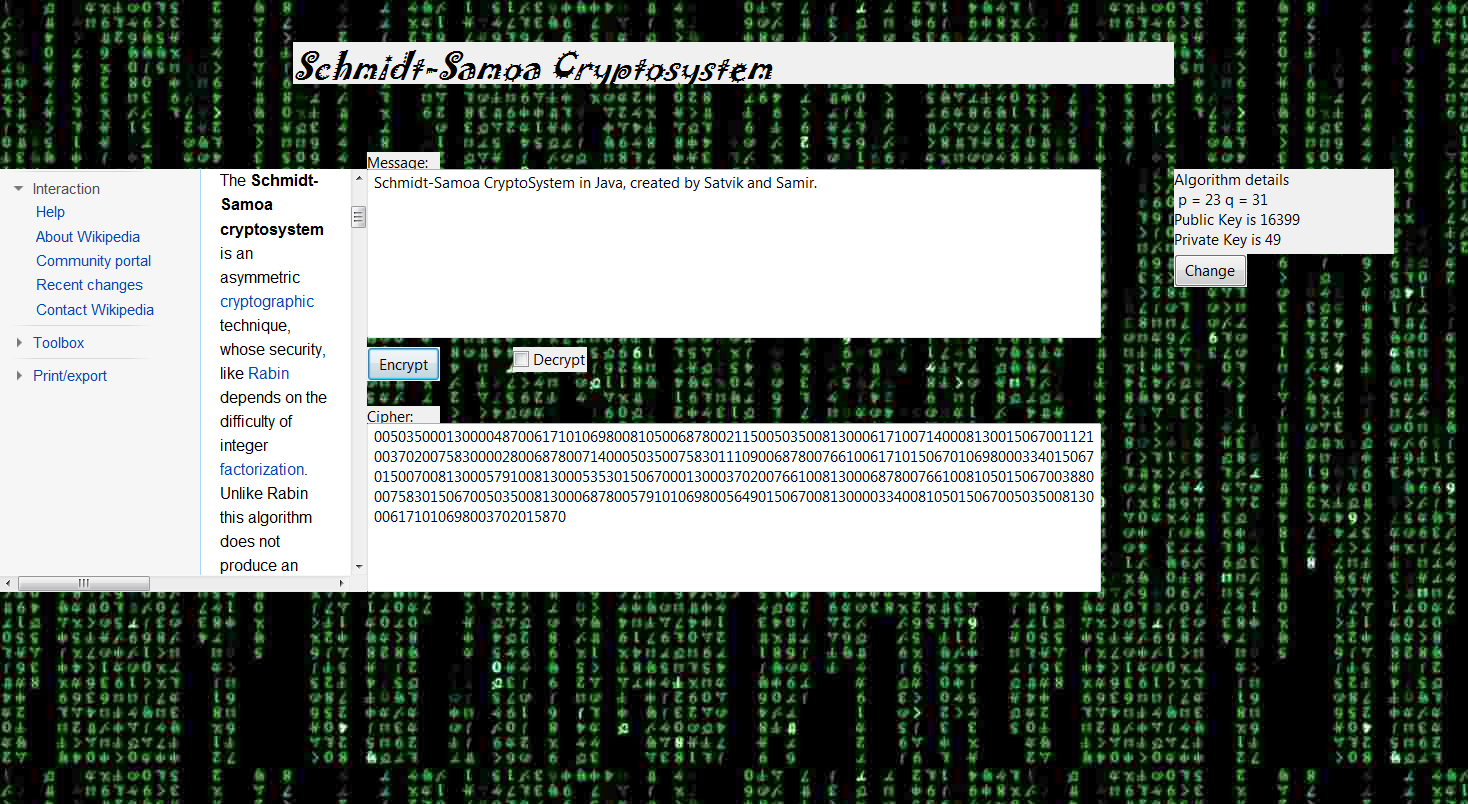
\includegraphics[scale=0.50]{encrypt.png}
  \caption{Encryption using the Schmidt-Samoa algorithm}
\end{figure}

\begin{figure}[h!]
  \centering
   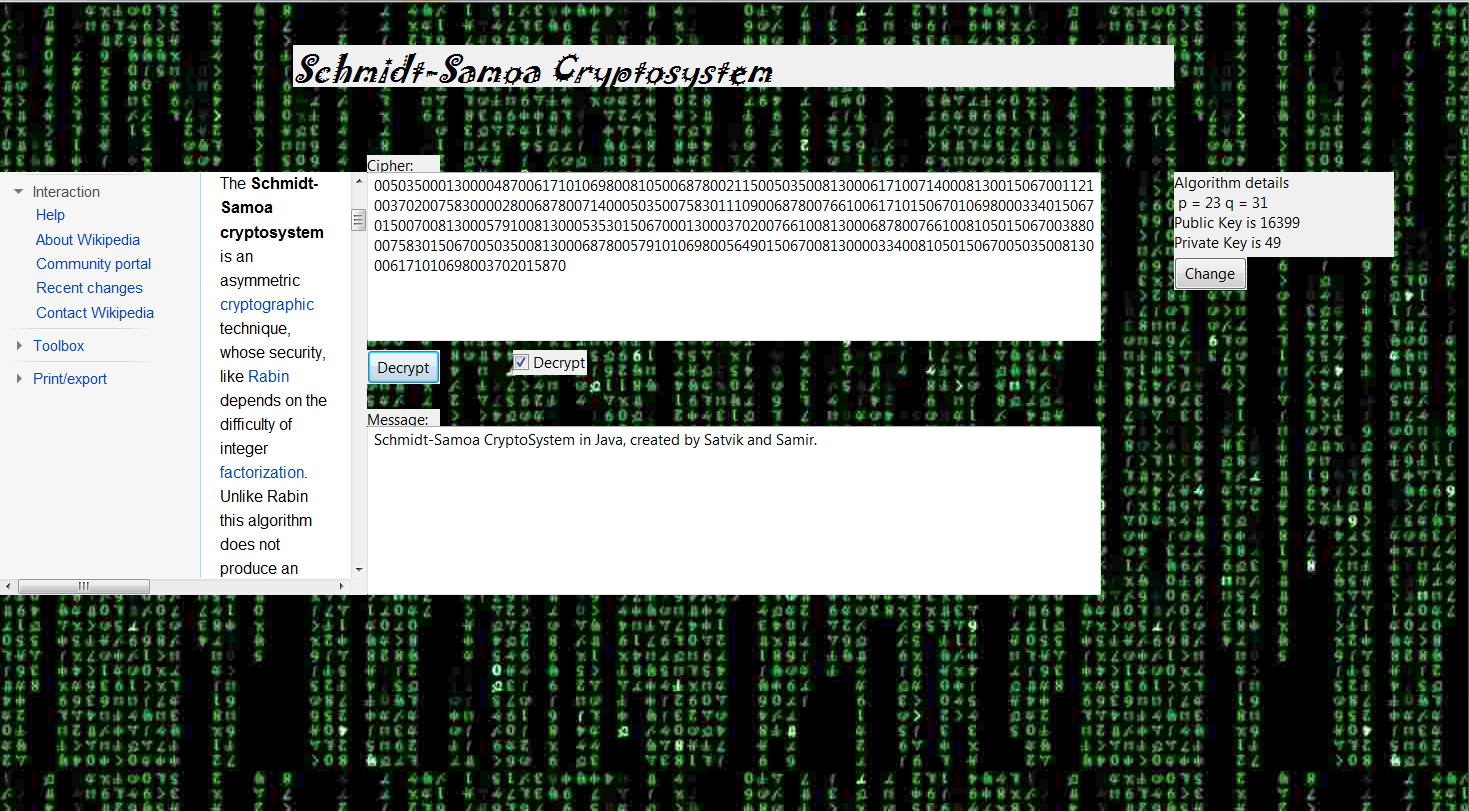
\includegraphics[scale=0.50]{decrypt.png}
  \caption{Decryption using the Schmidt-Samoa algorithm.}
\end{figure}


\end{document}
